\documentclass[a4paper,11pt]{article}
\usepackage{graphicx,url}
\usepackage[T1]{fontenc}
\usepackage[utf8]{inputenc}
\usepackage[brazil]{babel}
\usepackage{a4wide}
\usepackage{booktabs}
\graphicspath{{./imagens/}}
\usepackage{color} % the following is needed for syntax highlighting
\usepackage{listings} % For display code
\usepackage{mips} % MIPS highlighting for listings package

\definecolor{dkgreen}{rgb}{0,0.6,0}
\definecolor{gray}{rgb}{0.5,0.5,0.5}
\definecolor{mauve}{rgb}{0.58,0,0.82}

\lstset{
    language=[mips]Assembler,       % the language of the code
    basicstyle=\footnotesize,       % the size of the fonts that are used for the code
    numbers=left,                   % where to put the line-numbers
    numberstyle=\tiny\color{gray},  % the style that is used for the line-numbers
    stepnumber=1,                   % the step between two line-numbers. If it's 1, each line will be numbered
    numbersep=5pt,                  % how far the line-numbers are from the code
    backgroundcolor=\color{white},  % choose the background color. You must add \usepackage{color}
    showspaces=false,               % show spaces adding particular underscores
    showstringspaces=false,         % underline spaces within strings
    showtabs=false,                 % show tabs within strings adding particular underscores
    frame=single,                   % adds a frame around the code
    rulecolor=\color{black},        % if not set, the frame-color may be changed on line-breaks within not-black text (e.g. commens (green here))
    tabsize=4,                      % sets default tabsize to 4 spaces
    captionpos=b,                   % sets the caption-position to bottom
    breaklines=true,                % sets automatic line breaking
    breakatwhitespace=false,        % sets if automatic breaks should only happen at whitespace
    title=\lstname,                 % show the filename of files included with \lstinputlisting;
    % also try caption instead of title
    keywordstyle=\color{blue},          % keyword style
    commentstyle=\color{dkgreen},       % comment style
    stringstyle=\color{mauve},         % string literal style
    escapeinside={\%*}{*)},            % if you want to add a comment within your code
    morekeywords={*,...}               % if you want to add more keywords to the set
}

\title{\vspace{-4cm}Relatório 09 - Laboratório de Arquitetura de Computadores}
\author{Luiz Junio Veloso Dos Santos - Matricula: 624037}

\begin{document} 

\maketitle

\begin{enumerate}
    \item{Digite, compile e observe o programa a seguir:}
        \lstinputlisting{programa9.asm}
        \begin{enumerate}
            \item{Quando o programa é carregado, em quais posições de memória 
                    os dados foram armazenados?}

                \textbf{R: \underline{0x10010000} \underline{0x10010004} \underline{0x10010008}
                    \underline{0x1001000c}}

            \item{Complete o programa anterior de maneira a ler os valores armazenados em x1, x2, x3 e x4
                    em registradores (\$s1, \$s2, \$s3, \$s4)}

                \textbf{R: }
                \lstinputlisting{programa9b.asm}
                \newpage
            \item{Crie mais uma variável denominada soma e atribua um valor inicial de -1. A variável soma
                    deverá estar na posição seguinte a x4. Escrever um programa que leia todos os números, 
                    calcule e substitua o valor da variável soma por este valor.}

                \textbf{R: }
                \lstinputlisting{programa9c.asm}
        \end{enumerate}
        \newpage
    \item{Considere o seguinte programa: y = 127x – 65z + 1 \newline 
            Faça um programa que calcule o valor de y conhecendo os valores de x e z. 
            Os valores de x e z estão armazenados na memória e, na posição imediatamente a seguir, 
            o valor de y deverá ser escrito.}

        \textbf{R: }
        \lstinputlisting{programa10.asm}
        \newpage
    \item{Considere o seguinte programa: y = x – z + 300000 \newline 
            Faça um programa que calcule o valor de y conhecendo os valores de x e z. 
            Os valores de x e z estão armazenados na memória e, na posição imediatamente a seguir, 
            o valor de y deverá ser escrito.}

        \textbf{R: }
        \lstinputlisting{programa11.asm}
        \newpage
    \item{Considere a seguinte situação:\newline
            int ***x;\newline
            onde x contem um ponteiro para um ponteiro para um ponteiro para um inteiro.\newline 
            Nessa situação, considere que a posição inicial de memória contenha o inteiro em questão.
            Coloque todos os outros valores em registradores, use os endereços de memória que quiser 
            dentro do espaço de endereçamento do Mips.

            Resumo do problema:\newline
            k = MEM [ MEM [MEM [  x ] ] ].

            Crie um programa que crie a estrutura de dados acima, leia o  valor de K, dobre e 
            o reescreva conhecendo-se apenas o valor de x.}

        \textbf{R:}
        \lstinputlisting{programa12.asm}
\end{enumerate}

\newpage
\begin{figure}[!ht]
    \caption{Programa 9}
    \centering
    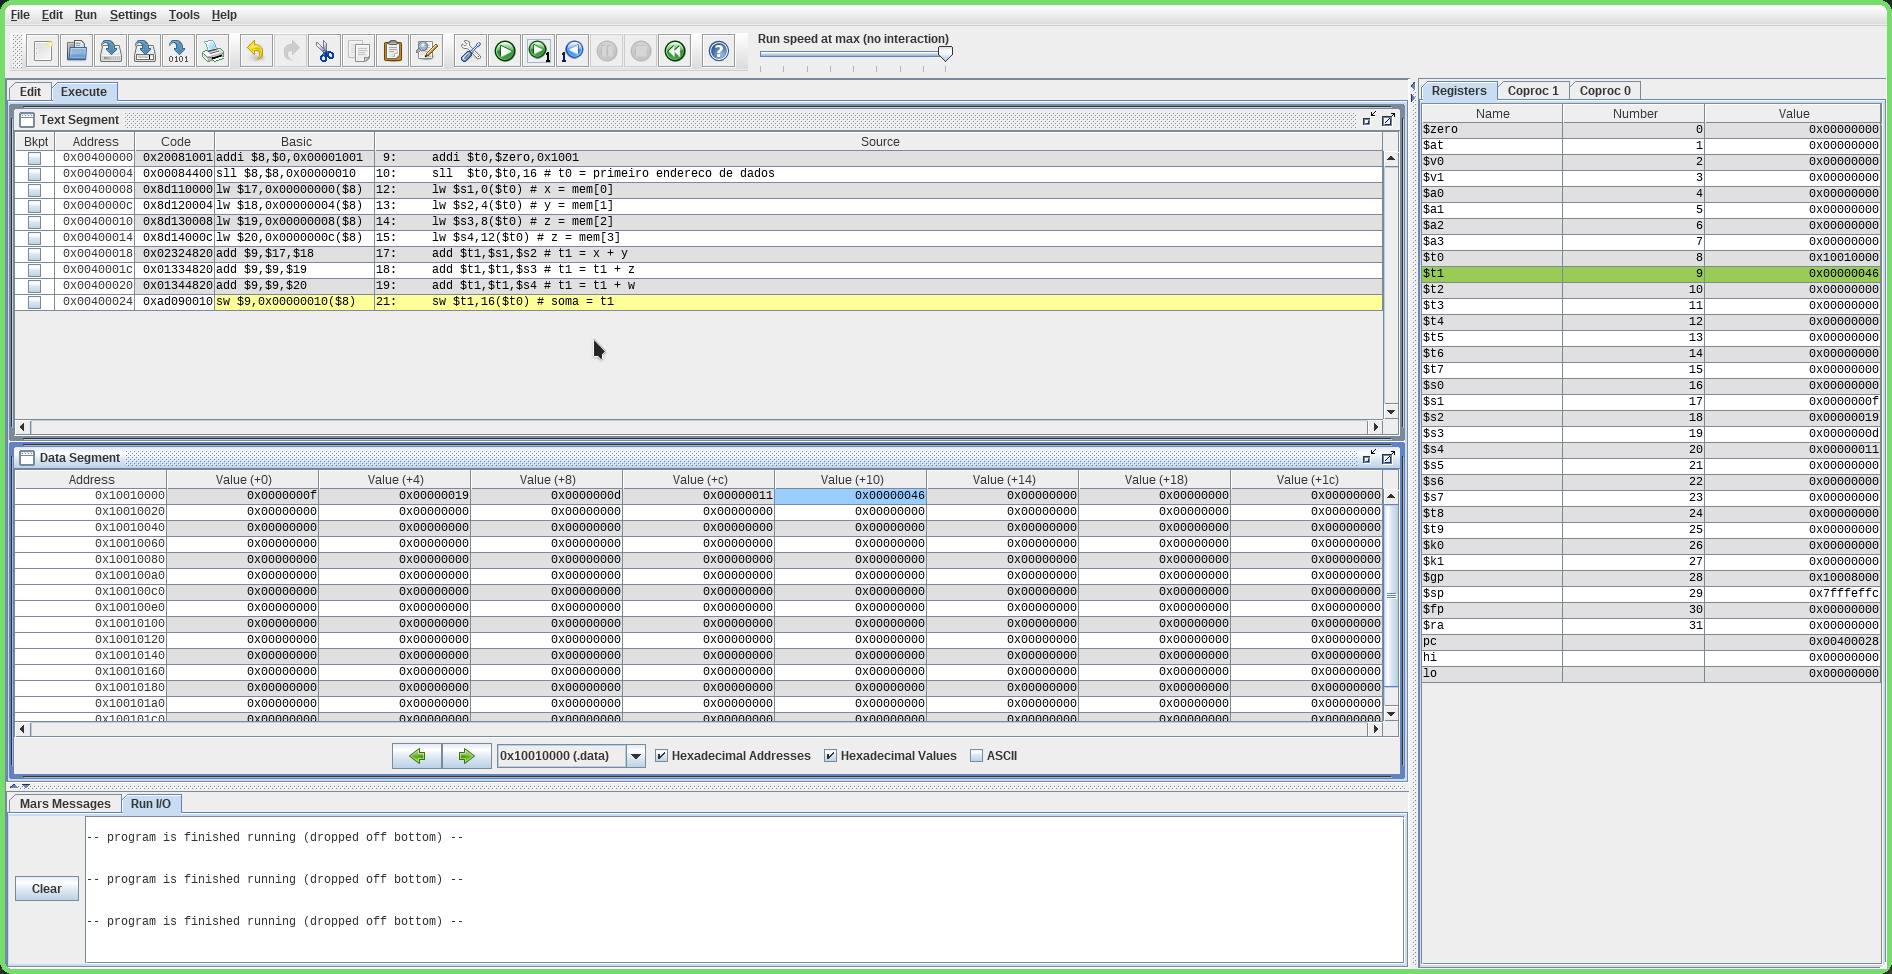
\includegraphics[width=1\textwidth]{programa9}
\end{figure}
\begin{figure}[!ht]
    \caption{Programa 10}
    \centering
    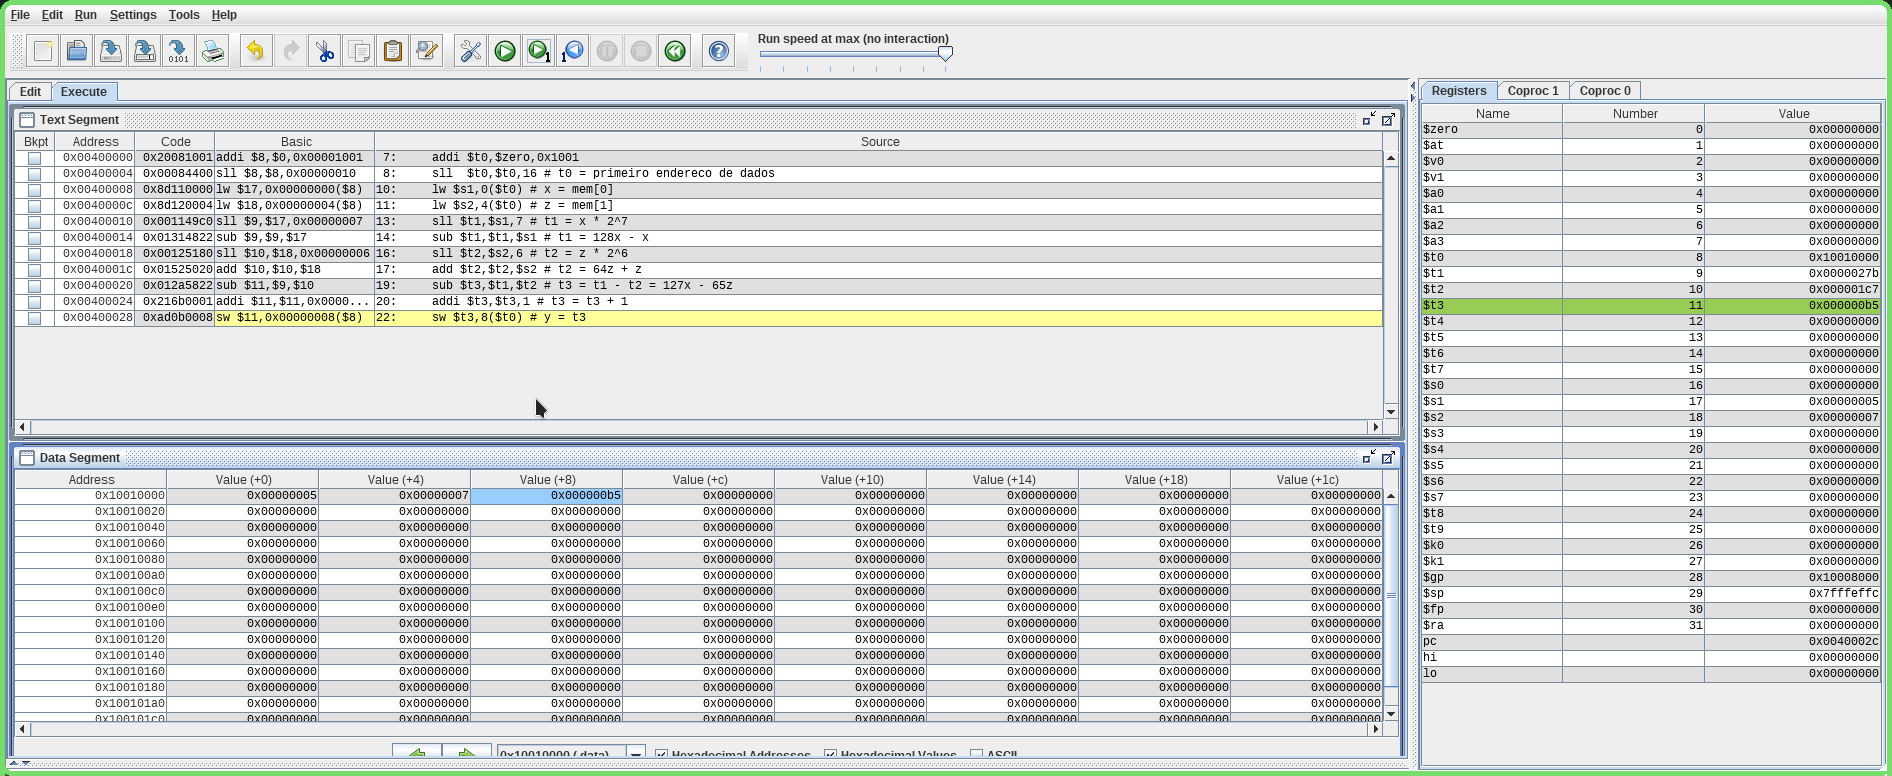
\includegraphics[width=1\textwidth]{programa10}
\end{figure}
\begin{figure}[!ht]
    \caption{Programa 11}
    \centering
    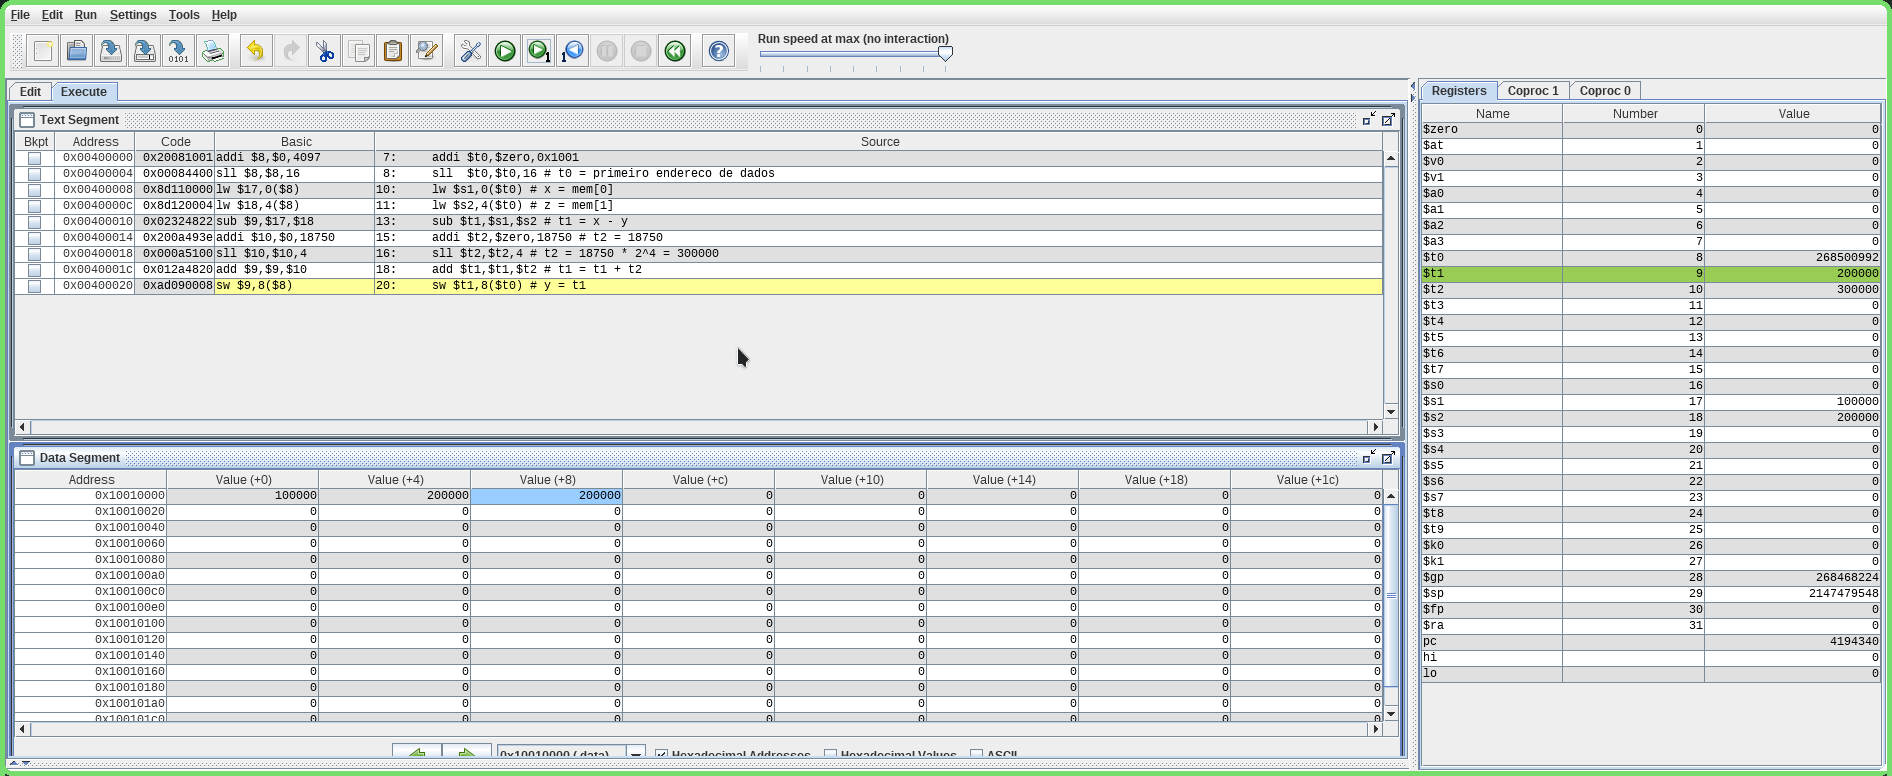
\includegraphics[width=1\textwidth]{programa11}
\end{figure} 
\begin{figure}[!ht]
    \caption{Programa 12}
    \centering
    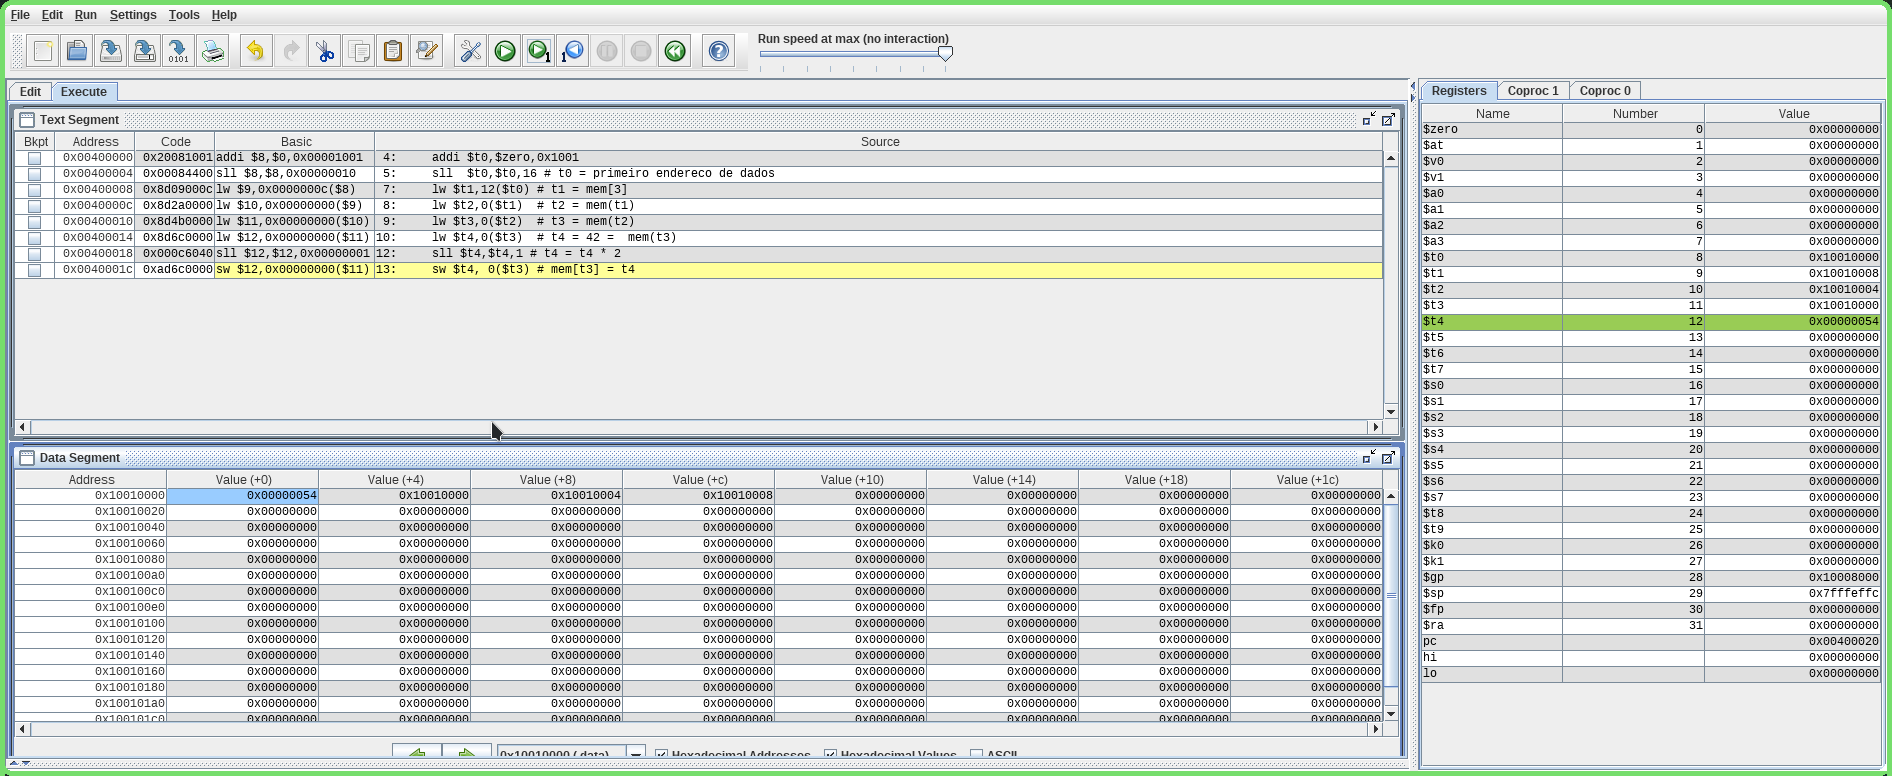
\includegraphics[width=1\textwidth]{programa12}
\end{figure} 

\end{document}
